\documentclass[aspectratio=169]{beamer}

%% ─── THEME & COLOR ──────────────────────────────────────────────────────────
\usetheme{Madrid}
\usecolortheme{default}

\definecolor{MandiGreen}{RGB}{34, 120, 80}
\definecolor{MandiDark}{RGB}{20, 60, 40}
\definecolor{MandiAccent}{RGB}{255, 160, 30}
\definecolor{AgentBlue}{RGB}{30, 100, 200}
\definecolor{AgentRed}{RGB}{200, 50, 50}
\definecolor{AgentPurple}{RGB}{130, 50, 180}
\definecolor{EnsembleGray}{RGB}{70, 70, 90}
\definecolor{LightGreen}{RGB}{210, 240, 220}
\definecolor{LightBlue}{RGB}{210, 230, 255}
\definecolor{LightYellow}{RGB}{255, 245, 210}
\definecolor{LightPurple}{RGB}{235, 220, 255}

\setbeamercolor{palette primary}{bg=MandiGreen, fg=white}
\setbeamercolor{palette secondary}{bg=MandiDark, fg=white}
\setbeamercolor{palette tertiary}{bg=MandiAccent, fg=black}
\setbeamercolor{title}{fg=MandiGreen}
\setbeamercolor{frametitle}{bg=MandiGreen, fg=white}
\setbeamercolor{structure}{fg=MandiGreen}
\setbeamercolor{block title}{bg=MandiGreen, fg=white}
\setbeamercolor{block body}{bg=LightGreen}
\setbeamercolor{alerted text}{fg=MandiAccent}
\setbeamercolor{footline}{bg=MandiDark, fg=white}

%% ─── PACKAGES ───────────────────────────────────────────────────────────────
\usepackage{tikz}
\usetikzlibrary{arrows.meta, positioning, shapes.geometric, fit, backgrounds, calc}
\usepackage{booktabs}
\usepackage{colortbl}
\usepackage{xcolor}
%\usepackage{fontawesome5} % not available; using text alternatives
\newcommand{\faArrowUp}{$\uparrow$}
\newcommand{\faArrowDown}{$\downarrow$}
\newcommand{\faShieldAlt}{[Shield]}
\newcommand{\faCheck}{[\checkmark]}
\newcommand{\faLock}{[Lock]}
\newcommand{\faExclamationTriangle}{[!]}
\newcommand{\faChartLine}{[\~{}]}
\usepackage{listings}
\usepackage{microtype}
\usepackage{graphicx}
\usepackage{array}
\usepackage{tabularx}

%% ─── LISTINGS STYLE ─────────────────────────────────────────────────────────
\lstdefinestyle{codestyle}{
  basicstyle=\ttfamily\tiny,
  keywordstyle=\color{MandiGreen}\bfseries,
  commentstyle=\color{gray}\itshape,
  stringstyle=\color{MandiAccent},
  backgroundcolor=\color{gray!10},
  frame=single,
  rulecolor=\color{MandiGreen!40},
  breaklines=true,
  showstringspaces=false,
}
\lstset{style=codestyle}

%% ─── TIKZ STYLES ─────────────────────────────────────────────────────────────
\tikzset{
  box/.style={rectangle, rounded corners=4pt, draw=#1, fill=#1!15,
              minimum width=2.2cm, minimum height=0.65cm,
              font=\scriptsize\bfseries, text=black, align=center},
  wbox/.style={rectangle, rounded corners=4pt, draw=#1, fill=white,
               minimum width=2.2cm, minimum height=0.65cm,
               font=\scriptsize\bfseries, text=#1, align=center},
  arr/.style={-{Stealth[length=5pt]}, thick, color=#1},
  grpbox/.style={rectangle, rounded corners=6pt, draw=#1, dashed,
                 fill=#1!5, inner sep=6pt},
  agentbox/.style={rectangle, rounded corners=4pt, draw=#1, fill=#1!20,
                   minimum width=2.8cm, minimum height=0.8cm,
                   font=\small\bfseries, text=black, align=center},
  smallbox/.style={rectangle, rounded corners=3pt, draw=#1, fill=#1!15,
                   minimum width=1.8cm, minimum height=0.55cm,
                   font=\tiny\bfseries, text=black, align=center},
}

%% ─── TITLE INFO ─────────────────────────────────────────────────────────────
\title[MandiSense AI]{\textbf{MandiSense AI}\\[4pt]
       \large Intelligent Agricultural Price Forecasting}
\subtitle{Multi-Agent Ensemble System — Phase 1 Review}
\author{BMS College of Engineering}
\date{\today}
\institute{Department of Computer Science \& Engineering}

%% ─────────────────────────────────────────────────────────────────────────────
\begin{document}

%% ── TITLE SLIDE ──────────────────────────────────────────────────────────────
\begin{frame}[plain]
\begin{tikzpicture}[remember picture, overlay]
  \fill[MandiGreen] (current page.north west) rectangle
       ([yshift=-2.2cm]current page.north east);
  \fill[MandiAccent] ([yshift=-2.2cm]current page.north west)
       rectangle ([yshift=-2.45cm]current page.north east);
  \fill[MandiDark] (current page.south west) rectangle
       ([yshift=1.2cm]current page.south east);
  \node[font=\huge\bfseries\color{white}, anchor=north] at
       ([yshift=-0.45cm]current page.north) {MandiSense AI};
  \node[font=\large\color{white!90}, anchor=north] at
       ([yshift=-1.3cm]current page.north)
       {Intelligent Agricultural Price Forecasting};
  \node[font=\small\color{white!80}, anchor=south] at
       ([yshift=0.5cm]current page.south)
       {BMS College of Engineering $\cdot$ Phase 1 Review $\cdot$ \today};
\end{tikzpicture}

\vspace{1.5cm}
\centering
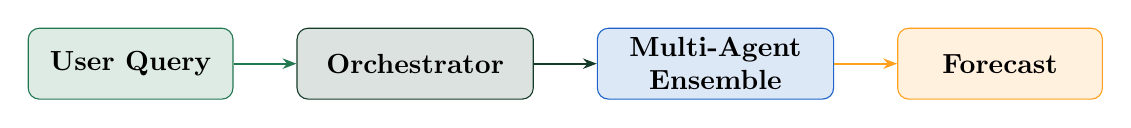
\begin{tikzpicture}
  \node[box=MandiGreen, minimum width=2.6cm, minimum height=0.9cm,
        font=\normalsize\bfseries] (q) {User Query};
  \node[box=MandiDark, minimum width=3cm, minimum height=0.9cm,
        font=\normalsize\bfseries, right=0.8cm of q] (o) {Orchestrator};
  \node[box=AgentBlue, minimum width=3cm, minimum height=0.9cm,
        font=\normalsize\bfseries, right=0.8cm of o] (e) {Multi-Agent\\Ensemble};
  \node[box=MandiAccent, minimum width=2.6cm, minimum height=0.9cm,
        font=\normalsize\bfseries, right=0.8cm of e] (r) {Forecast};
  \draw[arr=MandiGreen] (q) -- (o);
  \draw[arr=MandiDark] (o) -- (e);
  \draw[arr=MandiAccent] (e) -- (r);
\end{tikzpicture}

\vspace{0.4cm}
{\small \textit{"Tomato in Kolar Mandi" — End-to-End Trace}}
\end{frame}

%% ─────────────────────────────────────────────────────────────────────────────
%% SLIDE 1 — INTRODUCTION
%% ─────────────────────────────────────────────────────────────────────────────
% Speaker Notes: Welcome to the technical deep-dive of MandiSense AI. Today, we'll see exactly how our system handles a request for Tomato prices in Kolar. We've built a multi-agent system that mirrors how a real market expert thinks—looking at long-term trends, short-term arrivals, and external news.

\begin{frame}{MandiSense AI — Intelligent Agricultural Forecasting}
\begin{columns}[T]
  %% LEFT: Key Points
  \begin{column}{0.42\textwidth}
    \begin{block}{Mission}
      \begin{itemize}\setlength\itemsep{4pt}
        \item \textbf{Multi-Agent Ensemble} for Mandi Price Prediction
        \item Highly accurate, \textbf{interpretable} price forecasts
        \item Hybrid architecture: seasonality + supply shocks + external signals
        \item Case Study: \textit{"Tomato price for Kolar Mandi"}
      \end{itemize}
    \end{block}
    \vspace{0.3cm}
    \begin{block}{Code Entry Point}
      \begin{itemize}
        \item \texttt{run\_agents.py $\to$ main()}
      \end{itemize}
    \end{block}
  \end{column}
  %% RIGHT: Architecture Diagram
  \begin{column}{0.55\textwidth}
    \centering
    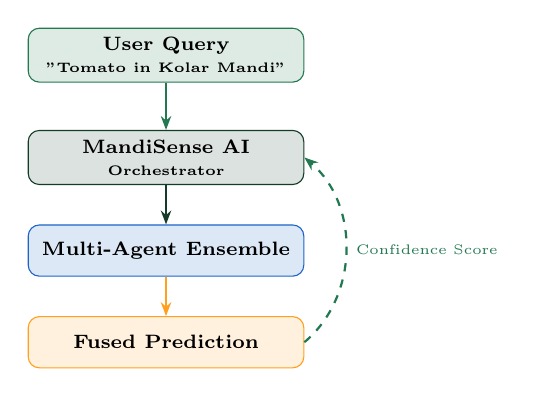
\begin{tikzpicture}[node distance=0.6cm]
      \node[box=MandiGreen, minimum width=3.5cm] (q) {User Query\\{\tiny "Tomato in Kolar Mandi"}};
      \node[box=MandiDark, minimum width=3.5cm, below=of q] (ai)
            {\textbf{MandiSense AI}\\{\tiny Orchestrator}};
      \node[box=AgentBlue, minimum width=3.5cm, below=0.5cm of ai] (mas)
            {Multi-Agent Ensemble};
      \node[box=MandiAccent, minimum width=3.5cm, below=0.5cm of mas] (out)
            {Fused Prediction};

      \draw[arr=MandiGreen] (q) -- (ai);
      \draw[arr=MandiDark]  (ai) -- (mas);
      \draw[arr=MandiAccent](mas) -- (out);

      % Feedback arrow
      \draw[arr=MandiGreen, dashed, bend right=50]
            (out.east) to node[right, font=\tiny, text=MandiGreen]
            {Confidence Score} (ai.east);
    \end{tikzpicture}
  \end{column}
\end{columns}
\end{frame}

%% ─────────────────────────────────────────────────────────────────────────────
%% SLIDE 2 — PROBLEM & OBJECTIVE
%% ─────────────────────────────────────────────────────────────────────────────
% Speaker Notes: Standard ML models often fail in agriculture because they treat everything as a single time series. Our objective is to split this complexity. We want to know: Is the price rising because it's 'Tomato Season', or because 'Kolar arrivals dropped'? This separation is key to our accuracy.

\begin{frame}{Problem \& Objective}
\begin{columns}[T]
  \begin{column}{0.48\textwidth}
    \begin{alertblock}{The Problem}
      \begin{itemize}\setlength\itemsep{3pt}
        \item Agricultural markets are \textbf{volatile}
        \item Disjoint factors: weather, festivals, supply
        \item Standard ML treats everything as one time series
        \item Cannot answer: \textit{"Why is Tomato expensive today?"}
      \end{itemize}
    \end{alertblock}
    \vspace{0.25cm}
    \begin{block}{The Objective}
      \begin{itemize}\setlength\itemsep{3pt}
        \item System that \textbf{reasons}, not just predicts
        \item 7-day and 30-day \textbf{explainable} forecasts
        \item Decompose complexity into specialist agents
      \end{itemize}
    \end{block}
    \vspace{0.15cm}
    \textbf{Code Mapping:}
    \begin{itemize}
      \item \texttt{SYSTEM\_CONTEXT.md} — Design philosophy
    \end{itemize}
  \end{column}
  \begin{column}{0.48\textwidth}
    \centering
    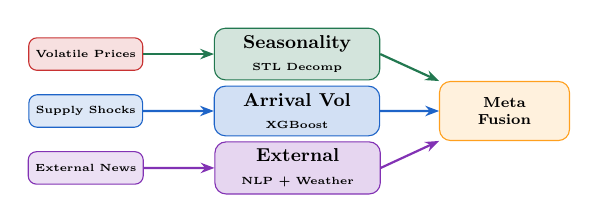
\begin{tikzpicture}[scale=0.75, transform shape, node distance=0.4cm]
      % Input signals
      \node[smallbox=AgentRed] (v) {Volatile Prices};
      \node[smallbox=AgentBlue, below=0.4cm of v] (s) {Supply Shocks};
      \node[smallbox=AgentPurple, below=0.4cm of s] (e) {External News};

      % Agents
      \node[agentbox=MandiGreen, right=1.2cm of v] (sa) {Seasonality\\{\tiny STL Decomp}};
      \node[agentbox=AgentBlue, right=1.2cm of s] (aa) {Arrival Vol\\{\tiny XGBoost}};
      \node[agentbox=AgentPurple, right=1.2cm of e] (ea) {External\\{\tiny NLP + Weather}};

      % Output
      \node[box=MandiAccent, minimum width=2.2cm, minimum height=1cm,
            right=1.0cm of aa] (out) {\textbf{Meta}\\Fusion};

      \draw[arr=MandiGreen] (v) -- (sa);
      \draw[arr=AgentBlue]  (s) -- (aa);
      \draw[arr=AgentPurple](e) -- (ea);

      \draw[arr=MandiGreen] (sa.east) -- (out.north west);
      \draw[arr=AgentBlue]  (aa.east) -- (out.west);
      \draw[arr=AgentPurple](ea.east) -- (out.south west);
    \end{tikzpicture}
  \end{column}
\end{columns}
\end{frame}

%% ─────────────────────────────────────────────────────────────────────────────
%% SLIDE 3 — SYSTEM ARCHITECTURE (COMPRESSED)
%% ─────────────────────────────────────────────────────────────────────────────
\begin{frame}{System Architecture Overview}
\centering
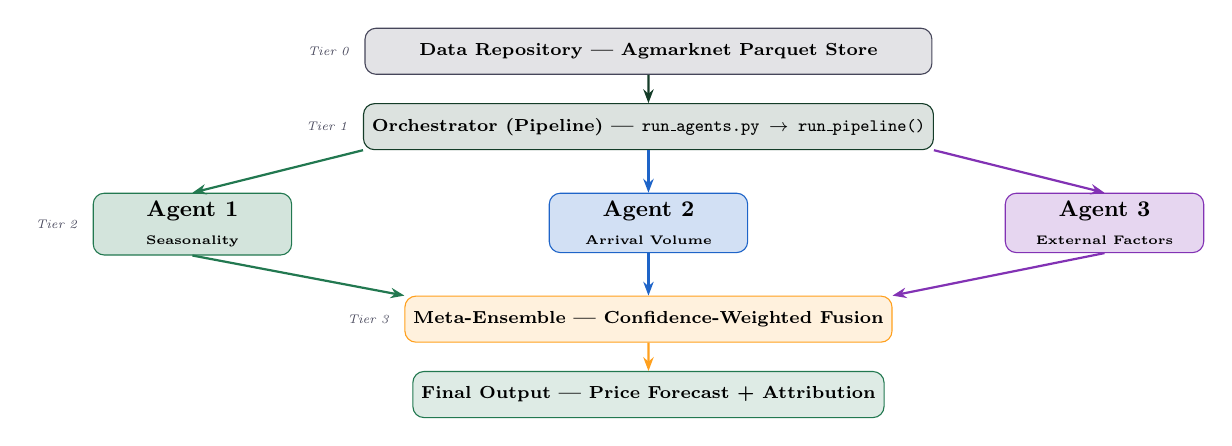
\begin{tikzpicture}[node distance=0.5cm and 0.3cm, scale=0.9, transform shape]

  %% DATA LAYER
  \node[box=EnsembleGray, minimum width=8cm] (data)
       {\textbf{Data Repository} — Agmarknet Parquet Store};

  %% ORCHESTRATOR
  \node[box=MandiDark, minimum width=8cm, below=0.4cm of data]
       (orch) {\textbf{Orchestrator (Pipeline)} — \texttt{run\_agents.py $\to$ run\_pipeline()}};

  \draw[arr=MandiDark] (data) -- (orch);

  %% THREE AGENTS (Compressed layout)
  \node[agentbox=MandiGreen, below left=0.6cm and 1cm of orch] (a1)
       {Agent 1\\{\tiny Seasonality}};
  \node[agentbox=AgentBlue, below=0.6cm of orch] (a2)
       {Agent 2\\{\tiny Arrival Volume}};
  \node[agentbox=AgentPurple, below right=0.6cm and 1cm of orch] (a3)
       {Agent 3\\{\tiny External Factors}};

  \draw[arr=MandiGreen] (orch.south west) -- (a1.north);
  \draw[arr=AgentBlue]  (orch.south)      -- (a2.north);
  \draw[arr=AgentPurple](orch.south east) -- (a3.north);

  %% META-ENSEMBLE
  \node[box=MandiAccent, minimum width=4.5cm, below=0.6cm of a2] (meta)
       {\textbf{Meta-Ensemble} — Confidence-Weighted Fusion};

  \draw[arr=MandiGreen] (a1.south) -- (meta.north west);
  \draw[arr=AgentBlue]  (a2.south) -- (meta.north);
  \draw[arr=AgentPurple](a3.south) -- (meta.north east);

  %% FINAL OUTPUT
  \node[box=MandiGreen, minimum width=4.5cm, below=0.4cm of meta] (out)
       {\textbf{Final Output} — Price Forecast + Attribution};

  \draw[arr=MandiAccent] (meta) -- (out);

  %% Tier labels
  \node[font=\tiny\itshape, text=EnsembleGray, left=0.1cm of data] {Tier 0};
  \node[font=\tiny\itshape, text=EnsembleGray, left=0.1cm of orch] {Tier 1};
  \node[font=\tiny\itshape, text=EnsembleGray, left=0.1cm of a1]   {Tier 2};
  \node[font=\tiny\itshape, text=EnsembleGray, left=0.1cm of meta] {Tier 3};

\end{tikzpicture}

\vspace{0.15cm}
\begin{columns}[T]
  \begin{column}{0.48\textwidth}
    \textbf{Code Mapping:}
    \begin{itemize}
      \item \texttt{mandisense\_ai/orchestrator/}
      \item \texttt{run\_agents.py $\to$ run\_pipeline()}
    \end{itemize}
  \end{column}
  \begin{column}{0.48\textwidth}
    \textbf{Key Properties:}
    \begin{itemize}
      \item Agents execute \textbf{in parallel}
      \item Each agent is \textbf{independently replaceable}
      \item Real-time UI via \textbf{WebSocket}
    \end{itemize}
  \end{column}
\end{columns}
\end{frame}

%% ─────────────────────────────────────────────────────────────────────────────
%% SLIDE 8 — EXTERNAL FACTORS AGENT (COMPRESSED/SPLIT VERTICALLY)
%% ─────────────────────────────────────────────────────────────────────────────
\begin{frame}{External Factors Agent — The News \& Weather Eye}
\begin{columns}[T]
  \begin{column}{0.42\textwidth}
    \begin{block}{Agent Goal}
      Capture \textbf{non-numeric} market impacts
    \end{block}
    \vspace{0.2cm}
    \begin{block}{Data Sources}
      \begin{itemize}\setlength\itemsep{3pt}
        \item \textbf{News scraper}: "Tomato Price Hike", "Rain damage"
        \item \textbf{Weather API}: Flood/drought alerts in Kolar region
        \item NLP Sentiment extraction
        \item Output: \textbf{Impact Score} $\in [-1.0, +1.0]$
      \end{itemize}
    \end{block}
    \vspace{0.2cm}
    \textbf{Code Mapping:}
    \begin{itemize}
      \item \texttt{external\_factors\_agent/\_\_init\_\_.py}\\
            \texttt{$\to$ run\_external\_factors\_agent()}
      \item \texttt{processing/external\_fusion.py}
    \end{itemize}
  \end{column}
  \begin{column}{0.55\textwidth}
    \centering
    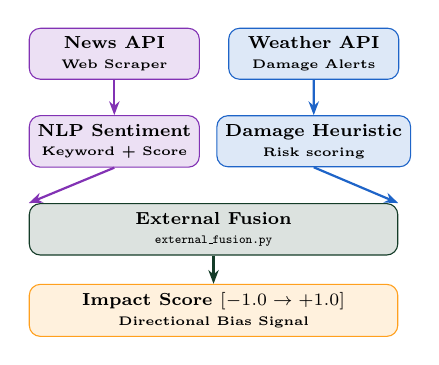
\begin{tikzpicture}[node distance=0.4cm, scale=0.9, transform shape]
      \node[box=AgentPurple, minimum width=2.4cm] (news)
           {News API\\{\tiny Web Scraper}};
      \node[box=AgentBlue, minimum width=2.4cm, right=0.4cm of news] (wx)
           {Weather API\\{\tiny Damage Alerts}};

      \node[box=AgentPurple, minimum width=2.4cm, below=0.5cm of news] (nlp)
           {\textbf{NLP Sentiment}\\{\tiny Keyword + Score}};
      \node[box=AgentBlue, minimum width=2.4cm, below=0.5cm of wx] (heur)
           {\textbf{Damage Heuristic}\\{\tiny Risk scoring}};

      \node[box=MandiDark, minimum width=5.2cm, below=0.5cm of nlp, xshift=1.4cm] (fuse)
           {\textbf{External Fusion}\\{\tiny \texttt{external\_fusion.py}}};

      \node[box=MandiAccent, minimum width=5.2cm, below=0.4cm of fuse] (out)
           {\textbf{Impact Score} $[-1.0 \to +1.0]$\\{\tiny Directional Bias Signal}};

      \draw[arr=AgentPurple](news) -- (nlp);
      \draw[arr=AgentBlue]  (wx)   -- (heur);
      \draw[arr=AgentPurple](nlp.south)  -- (fuse.north west);
      \draw[arr=AgentBlue]  (heur.south) -- (fuse.north east);
      \draw[arr=MandiDark]  (fuse) -- (out);
    \end{tikzpicture}
  \end{column}
\end{columns}
\end{frame}

%% ─────────────────────────────────────────────────────────────────────────────
%% SLIDE 9 — AGENT OUTPUTS COMPARISON (DIAGRAM BELOW TABLE)
%% ─────────────────────────────────────────────────────────────────────────────
\begin{frame}{Agent Outputs — Comparison \& Conflict}
\vspace{0.1cm}
\begin{columns}[T]
  \begin{column}{0.5\textwidth}
    \centering
    \renewcommand{\arraystretch}{1.4}
    \begin{tabular}{|>{\bfseries}l|c|c|c|}
      \hline
      \rowcolor{MandiGreen!80}
      \color{white}Agent &
      \color{white}Pred. &
      \color{white}Conf. &
      \color{white}Signal \\
      \hline
      \rowcolor{LightGreen}
      Seasonality & \textcolor{MandiGreen}{\textbf{+8\%}} & 0.85 &
        \textcolor{MandiGreen}{\faArrowUp\ Bullish} \\
      \hline
      \rowcolor{LightBlue}
      Arrival Vol & \textcolor{AgentRed}{\textbf{-3\%}} & 0.70 &
        \textcolor{AgentRed}{\faArrowDown\ Bearish} \\
      \hline
      \rowcolor{LightPurple}
      External & \textcolor{AgentPurple}{\textbf{+2\%}} & 0.40 &
        \textcolor{AgentPurple}{\faArrowUp\ Positive} \\
      \hline
    \end{tabular}

    \vspace{0.3cm}
    \begin{alertblock}{\faExclamationTriangle\ Conflict Detected}
      Seasonality (+8\%) \textbf{vs.} Arrival (-3\%)\\
      \textit{High-confidence agents disagree on direction!}
    \end{alertblock}
  \end{column}
  \begin{column}{0.46\textwidth}
    \textbf{Code Mapping:}
    \begin{itemize}
      \item \texttt{run\_agents.py} Lines 31–47
      \item Captures \texttt{seasonality\_output},\\
            \texttt{arrival\_output},\\
            \texttt{external\_impact}
    \end{itemize}
    \vspace{0.4cm}
    \centering
    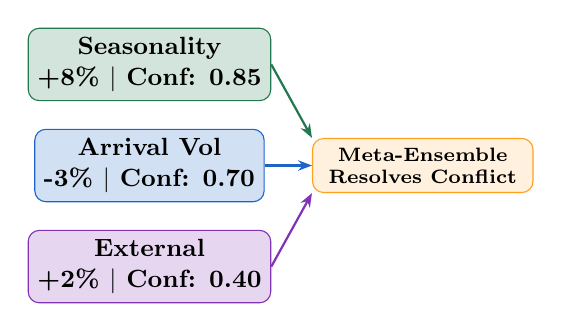
\begin{tikzpicture}[node distance=0.35cm]
      \node[agentbox=MandiGreen, minimum width=2.6cm] (sa) {Seasonality\\+8\% $|$ Conf: 0.85};
      \node[agentbox=AgentBlue, minimum width=2.6cm, below=0.35cm of sa] (aa)
            {Arrival Vol\\-3\% $|$ Conf: 0.70};
      \node[agentbox=AgentPurple, minimum width=2.6cm, below=0.35cm of aa] (ea)
            {External\\+2\% $|$ Conf: 0.40};

      \node[box=MandiAccent, minimum width=2.8cm, right=0.6cm of aa] (ens) 
            {\textbf{Meta-Ensemble}\\Resolves Conflict};

      \draw[arr=MandiGreen] (sa.east) -- (ens.north west);
      \draw[arr=AgentBlue]  (aa.east) -- (ens.west);
      \draw[arr=AgentPurple](ea.east) -- (ens.south west);
    \end{tikzpicture}
  \end{column}
\end{columns}
\end{frame}

%% ─────────────────────────────────────────────────────────────────────────────
%% SLIDE 10 — META-ENSEMBLE FUSION (STACKED VERSION)
%% ─────────────────────────────────────────────────────────────────────────────
\begin{frame}{Meta-Ensemble — Confidence-Aware Fusion}
\begin{columns}[T]
  \begin{column}{0.45\textwidth}
    \begin{block}{Fusion Logic}
      \begin{itemize}\setlength\itemsep{3pt}
        \item \textbf{Dynamic Weighting}: High-confidence agent gets more weight
        \item \textbf{Arrival Boost}: If supply stress is critical, $w_2$ is amplified
        \item \textbf{Horizon Alignment}: Normalises 30-day seasonal to 7-day scale
        \item External acts as a \textbf{directional bias}, not a forecast
      \end{itemize}
    \end{block}
    \vspace{0.2cm}
    \textbf{Code Mapping:}
    \begin{itemize}
      \item \texttt{meta\_ensemble.py $\to$ fuse()} (Line 192)
      \item \texttt{\_SEASONALITY\_HORIZON\_DAYS} — alignment constant
    \end{itemize}
  \end{column}
  \begin{column}{0.52\textwidth}
    \centering
    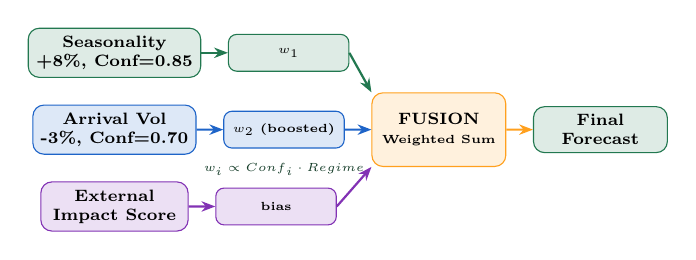
\begin{tikzpicture}[scale=0.85, transform shape, node distance=0.35cm]
      \node[box=MandiGreen, minimum width=2.2cm] (sa)
           {Seasonality\\+8\%, Conf=0.85};
      \node[box=AgentBlue, minimum width=2.2cm, below=0.4cm of sa] (aa)
           {Arrival Vol\\-3\%, Conf=0.70};
      \node[box=AgentPurple, minimum width=2.2cm, below=0.4cm of aa] (ea)
           {External\\Impact Score};

      \node[smallbox=MandiGreen, right=0.4cm of sa] (w1) {$w_1$};
      \node[smallbox=AgentBlue, right=0.4cm of aa]  (w2) {$w_2$ \tiny(boosted)};
      \node[smallbox=AgentPurple, right=0.4cm of ea] (b)  {bias};

      \node[box=MandiAccent, minimum width=2cm, minimum height=1.1cm,
            right=0.4cm of w2] (fuse) {\textbf{FUSION}\\{\tiny Weighted Sum}};

      \node[box=MandiGreen, minimum width=2cm, right=0.4cm of fuse] (out)
           {\textbf{Final}\\\textbf{Forecast}};

      \draw[arr=MandiGreen] (sa) -- (w1);
      \draw[arr=AgentBlue]  (aa) -- (w2);
      \draw[arr=AgentPurple](ea) -- (b);

      \draw[arr=MandiGreen] (w1.east) -- (fuse.north west);
      \draw[arr=AgentBlue]  (w2.east) -- (fuse.west);
      \draw[arr=AgentPurple](b.east)  -- (fuse.south west);

      \draw[arr=MandiAccent](fuse) -- (out);

      \node[font=\tiny\itshape, text=MandiDark, below=0.1cm of w2]
           {$w_i \propto \text{Conf}_i \cdot \text{Regime}$};
    \end{tikzpicture}
  \end{column}
\end{columns}
\end{frame}

%% ─────────────────────────────────────────────────────────────────────────────
%% SLIDE 11 — CONFLICT HANDLING (COMPRESSED)
%% ─────────────────────────────────────────────────────────────────────────────
\begin{frame}{Conflict Handling — The Safety Net}
\begin{columns}[T]
  \begin{column}{0.40\textwidth}
    \begin{alertblock}{Conflict Detection Logic}
      \begin{itemize}\setlength\itemsep{3pt}
        \item Two \textbf{high-confidence} agents point in \textbf{opposite directions}
        \item System \textbf{dampens} the result
        \item Prevents extreme, risky predictions
        \item Sets \texttt{conflict\_detected=True} for UI
      \end{itemize}
    \end{alertblock}
    \vspace{0.2cm}
    \begin{block}{Design Principle}
      \textit{"We'd rather be slightly wrong than confidently wrong."}
    \end{block}
    \vspace{0.2cm}
    \textbf{Code Mapping:}
    \begin{itemize}
      \item \texttt{meta\_ensemble.py}\\
            \texttt{$\to$ \_CONFLICT\_SIGN\_THRESHOLD}
      \item \texttt{$\to$ \_CONFLICT\_DAMPEN\_FACTOR\_NORMAL}
    \end{itemize}
  \end{column}
  \begin{column}{0.57\textwidth}
    \centering
    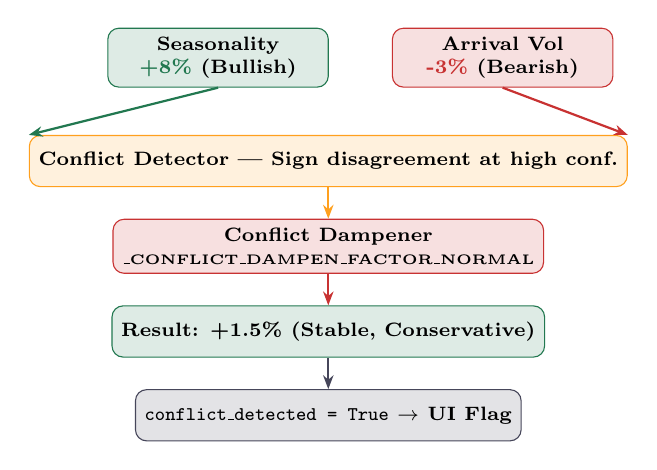
\begin{tikzpicture}[node distance=0.5cm]
      \node[box=MandiGreen, minimum width=2.8cm] (sa)
           {Seasonality\\{\textcolor{MandiGreen}{\textbf{+8\%}}} (Bullish)};
      \node[box=AgentRed, minimum width=2.8cm, right=0.8cm of sa] (aa)
           {Arrival Vol\\{\textcolor{AgentRed}{\textbf{-3\%}}} (Bearish)};

      \node[box=MandiAccent, minimum width=6.4cm, below=0.6cm of sa, xshift=1.4cm] (det)
           {\textbf{Conflict Detector} — Sign disagreement at high conf.};

      \node[box=AgentRed, minimum width=4cm, below=0.4cm of det] (damp)
           {\textbf{Conflict Dampener}\\{\tiny \_CONFLICT\_DAMPEN\_FACTOR\_NORMAL}};

      \node[box=MandiGreen, minimum width=4cm, below=0.4cm of damp] (res)
           {\textbf{Result: +1.5\%} (Stable, Conservative)};

      \node[box=EnsembleGray, minimum width=3.5cm, below=0.4cm of res] (flag)
           {\texttt{conflict\_detected = True} $\to$ UI Flag};

      \draw[arr=MandiGreen] (sa.south) -- (det.north west);
      \draw[arr=AgentRed]   (aa.south) -- (det.north east);
      \draw[arr=MandiAccent](det)  -- (damp);
      \draw[arr=AgentRed]   (damp) -- (res);
      \draw[arr=EnsembleGray](res) -- (flag);
    \end{tikzpicture}
  \end{column}
\end{columns}
\end{frame}

%% ─────────────────────────────────────────────────────────────────────────────
%% SLIDE 12 — FINAL PREDICTION GENERATION (FIXED NODE POSITIONS)
%% ─────────────────────────────────────────────────────────────────────────────
\begin{frame}{Agent Outputs — Comparison \& Conflict}
\vspace{0.1cm}
\begin{columns}[T]
  \begin{column}{0.5\textwidth}
    \centering
    \renewcommand{\arraystretch}{1.4}
    \begin{tabular}{|>{\bfseries}l|c|c|c|}
      \hline
      \rowcolor{MandiGreen!80}
      \color{white}Agent &
      \color{white}Pred. &
      \color{white}Conf. &
      \color{white}Signal \\
      \hline
      \rowcolor{LightGreen}
      Seasonality & \textcolor{MandiGreen}{\textbf{+8\%}} & 0.85 &
        \textcolor{MandiGreen}{\faArrowUp\ Bullish} \\
      \hline
      \rowcolor{LightBlue}
      Arrival Vol & \textcolor{AgentRed}{\textbf{-3\%}} & 0.70 &
        \textcolor{AgentRed}{\faArrowDown\ Bearish} \\
      \hline
      \rowcolor{LightPurple}
      External & \textcolor{AgentPurple}{\textbf{+2\%}} & 0.40 &
        \textcolor{AgentPurple}{\faArrowUp\ Positive} \\
      \hline
    \end{tabular}

    \vspace{0.3cm}
    \begin{alertblock}{\faExclamationTriangle\ Conflict Detected}
      Seasonality (+8\%) \textbf{vs.} Arrival (-3\%)\\
      \textit{High-confidence agents disagree on direction!}
    \end{alertblock}
  \end{column}
  \begin{column}{0.46\textwidth}
    \textbf{Code Mapping:}
    \begin{itemize}
      \item \texttt{run\_agents.py} Lines 31–47
      \item Captures \texttt{seasonality\_output},\\
            \texttt{arrival\_output},\\
            \texttt{external\_impact}
    \end{itemize}
    \vspace{0.4cm}
    \centering
    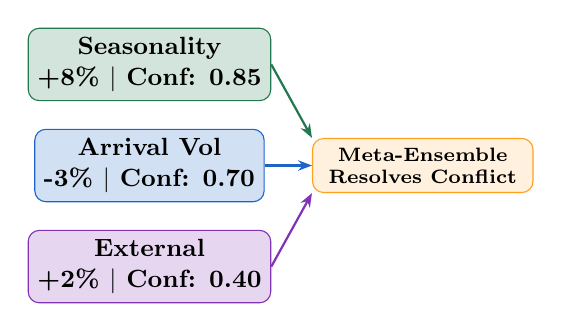
\begin{tikzpicture}[node distance=0.35cm]
      \node[agentbox=MandiGreen, minimum width=2.6cm] (sa) {Seasonality\\+8\% $|$ Conf: 0.85};
      \node[agentbox=AgentBlue, minimum width=2.6cm, below=0.35cm of sa] (aa)
            {Arrival Vol\\-3\% $|$ Conf: 0.70};
      \node[agentbox=AgentPurple, minimum width=2.6cm, below=0.35cm of aa] (ea)
            {External\\+2\% $|$ Conf: 0.40};

      \node[box=MandiAccent, minimum width=2.8cm, right=0.6cm of aa] (ens) 
            {\textbf{Meta-Ensemble}\\Resolves Conflict};

      \draw[arr=MandiGreen] (sa.east) -- (ens.north west);
      \draw[arr=AgentBlue]  (aa.east) -- (ens.west);
      \draw[arr=AgentPurple](ea.east) -- (ens.south west);
    \end{tikzpicture}
  \end{column}
\end{columns}
\end{frame}

%% ─────────────────────────────────────────────────────────────────────────────
%% SLIDE 14 — SYSTEM STRENGTHS (FIXED vs. POSITIONING)
%% ─────────────────────────────────────────────────────────────────────────────
\begin{frame}{Final Prediction Generation}
\begin{columns}[T]
  \begin{column}{0.48\textwidth}
    \begin{block}{Prediction Output}
      \begin{itemize}\setlength\itemsep{4pt}
        \item \textbf{Numerical Fusion}: Final \% change calculated
        \item \textbf{Confidence}: Aggregated with conflict penalty applied
        \item \textbf{Attribution}: Explains \textit{which} agent drove the result
      \end{itemize}
    \end{block}
    \vspace{0.2cm}
    \begin{exampleblock}{\faChartLine\ Sample Output — Tomato / Kolar}
      \begin{itemize}
        \item Prediction: \textbf{+4.2\%}
        \item Confidence: \textbf{78\%}
        \item \textcolor{AgentBlue}{Supply (Arrival): 65\%}
        \item \textcolor{MandiGreen}{Trend (Seasonal): 25\%}
        \item \textcolor{AgentPurple}{News (External): 10\%}
      \end{itemize}
    \end{exampleblock}
  \end{column}
  \begin{column}{0.48\textwidth}
    \centering
    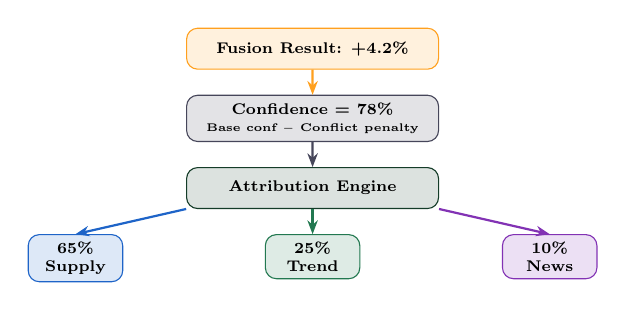
\begin{tikzpicture}[scale=0.8, transform shape, node distance=0.4cm]
      \node[box=MandiAccent, minimum width=4cm] (fuse)
           {\textbf{Fusion Result: +4.2\%}};

      \node[box=EnsembleGray, minimum width=4cm, below=0.4cm of fuse] (conf)
           {Confidence = 78\%\\{\tiny Base conf $-$ Conflict penalty}};

      \node[box=MandiDark, minimum width=4cm, below=0.4cm of conf] (attr)
           {\textbf{Attribution Engine}};

      \node[box=AgentBlue, minimum width=1.5cm, below left=0.4cm and 1cm of attr] (a1)
           {\textbf{65\%}\\Supply};
      \node[box=MandiGreen, minimum width=1.5cm, below=0.4cm of attr] (a2)
           {\textbf{25\%}\\Trend};
      \node[box=AgentPurple, minimum width=1.5cm, below right=0.4cm and 1cm of attr] (a3)
           {\textbf{10\%}\\News};

      \draw[arr=MandiAccent](fuse) -- (conf);
      \draw[arr=EnsembleGray](conf) -- (attr);
      \draw[arr=AgentBlue]   (attr.south west) -- (a1.north);
      \draw[arr=MandiGreen]  (attr.south)      -- (a2.north);
      \draw[arr=AgentPurple] (attr.south east) -- (a3.north);
    \end{tikzpicture}
  \end{column}
\end{columns}
\end{frame}

%% ─────────────────────────────────────────────────────────────────────────────
%% SLIDE 15 — CONCLUSION & FUTURE OUTLOOK (UNCHANGED)
%% ─────────────────────────────────────────────────────────────────────────────
\begin{frame}{Conclusion \& Future Outlook}
\begin{columns}[T]
  \begin{column}{0.44\textwidth}
    \begin{block}{Current State}
      \begin{itemize}\setlength\itemsep{4pt}
        \item Stable \textbf{3-agent ensemble} for 5+ commodities
        \item Full end-to-end pipeline from query to decision
        \item Conflict-aware, confidence-weighted fusion
        \item Explainable attribution at every level
      \end{itemize}
    \end{block}
    \vspace{0.2cm}
    \begin{exampleblock}{Future Roadmap}
      \begin{itemize}\setlength\itemsep{3pt}
        \item \textbf{Causal Inference} — "Why exactly?"
        \item \textbf{LLM Reasoning Traces} — Natural language explanations
        \item More commodities, more mandis
      \end{itemize}
    \end{exampleblock}
    \vspace{0.15cm}
    \textbf{Code Mapping:}
    \begin{itemize}
      \item \texttt{SYSTEM\_HANDOFF.md} — Future agent roadmap
    \end{itemize}
  \end{column}
  \begin{column}{0.53\textwidth}
    \centering
    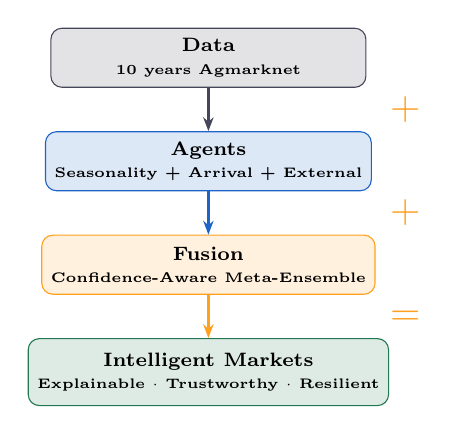
\begin{tikzpicture}[node distance=0.55cm]
      \node[box=EnsembleGray, minimum width=4cm, minimum height=0.75cm] (d)
           {\textbf{Data}\\{\tiny 10 years Agmarknet}};
      \node[box=AgentBlue, minimum width=4cm, minimum height=0.75cm, below=of d] (a)
           {\textbf{Agents}\\{\tiny Seasonality + Arrival + External}};
      \node[box=MandiAccent, minimum width=4cm, minimum height=0.75cm, below=of a] (f)
           {\textbf{Fusion}\\{\tiny Confidence-Aware Meta-Ensemble}};
      \node[box=MandiGreen, minimum width=4cm, minimum height=0.85cm, below=of f] (r)
           {\textbf{Intelligent Markets}\\{\tiny Explainable $\cdot$ Trustworthy $\cdot$ Resilient}};

      \draw[arr=EnsembleGray](d) -- (a);
      \draw[arr=AgentBlue]   (a) -- (f);
      \draw[arr=MandiAccent] (f) -- (r);

      \node[font=\Large, text=MandiAccent] at ($(d)!0.5!(a) + (2.5,0)$) {+};
      \node[font=\Large, text=MandiAccent] at ($(a)!0.5!(f) + (2.5,0)$) {+};
      \node[font=\Large, text=MandiAccent] at ($(f)!0.5!(r) + (2.5,0)$) {=};
    \end{tikzpicture}

    \vspace{0.4cm}
    \begin{center}
      {\large\itshape ``MandiSense AI is the intersection of}\\
      {\large\itshape Data Science and Domain Expertise.''}
    \end{center}
  \end{column}
\end{columns}
\end{frame}

%% ─── THANK YOU SLIDE ─────────────────────────────────────────────────────────
\begin{frame}[plain]
\begin{tikzpicture}[remember picture, overlay]
  \fill[MandiGreen] (current page.north west) rectangle (current page.south east);
  \fill[MandiDark, opacity=0.4]
       (current page.south west) rectangle ([yshift=3cm]current page.south east);
  \node[font=\Huge\bfseries\color{white}] at (current page.center)
       {Thank You};
  \node[font=\large\color{white!80}, below=0.6cm of current page.center]
       {MandiSense AI — Phase 1 Review};
  \node[font=\normalsize\color{MandiAccent}, below=1.4cm of current page.center]
       {BMS College of Engineering};
\end{tikzpicture}
\end{frame}

\end{document}